\chapter{查询处理}

\begin{introduction}[期末考试提纲]
    \item 三种连接算法的实现策略及各自适用场合
\end{introduction}

\section{查询处理流程}

\begin{definition}[查询处理]
    查询处理是指从数据库中提取数据的一系列活动, 主要包括:
    \begin{itemize}
        \item 将用高层数据库语言表示的查询语句翻译为能在文件系统这一物理层次上实现的表达式;
        \item 为优化查询而进行各种转换;
        \item 查询的实际执行.
    \end{itemize}
    实际上就是实现一个
    \begin{itemize}
        \item 输入: SQL语句
        \item 输出: 满足查询条件的数据
    \end{itemize}
    的过程.
\end{definition}


\subsection{查询处理步骤}


\begin{figure}[H]
    \centering
    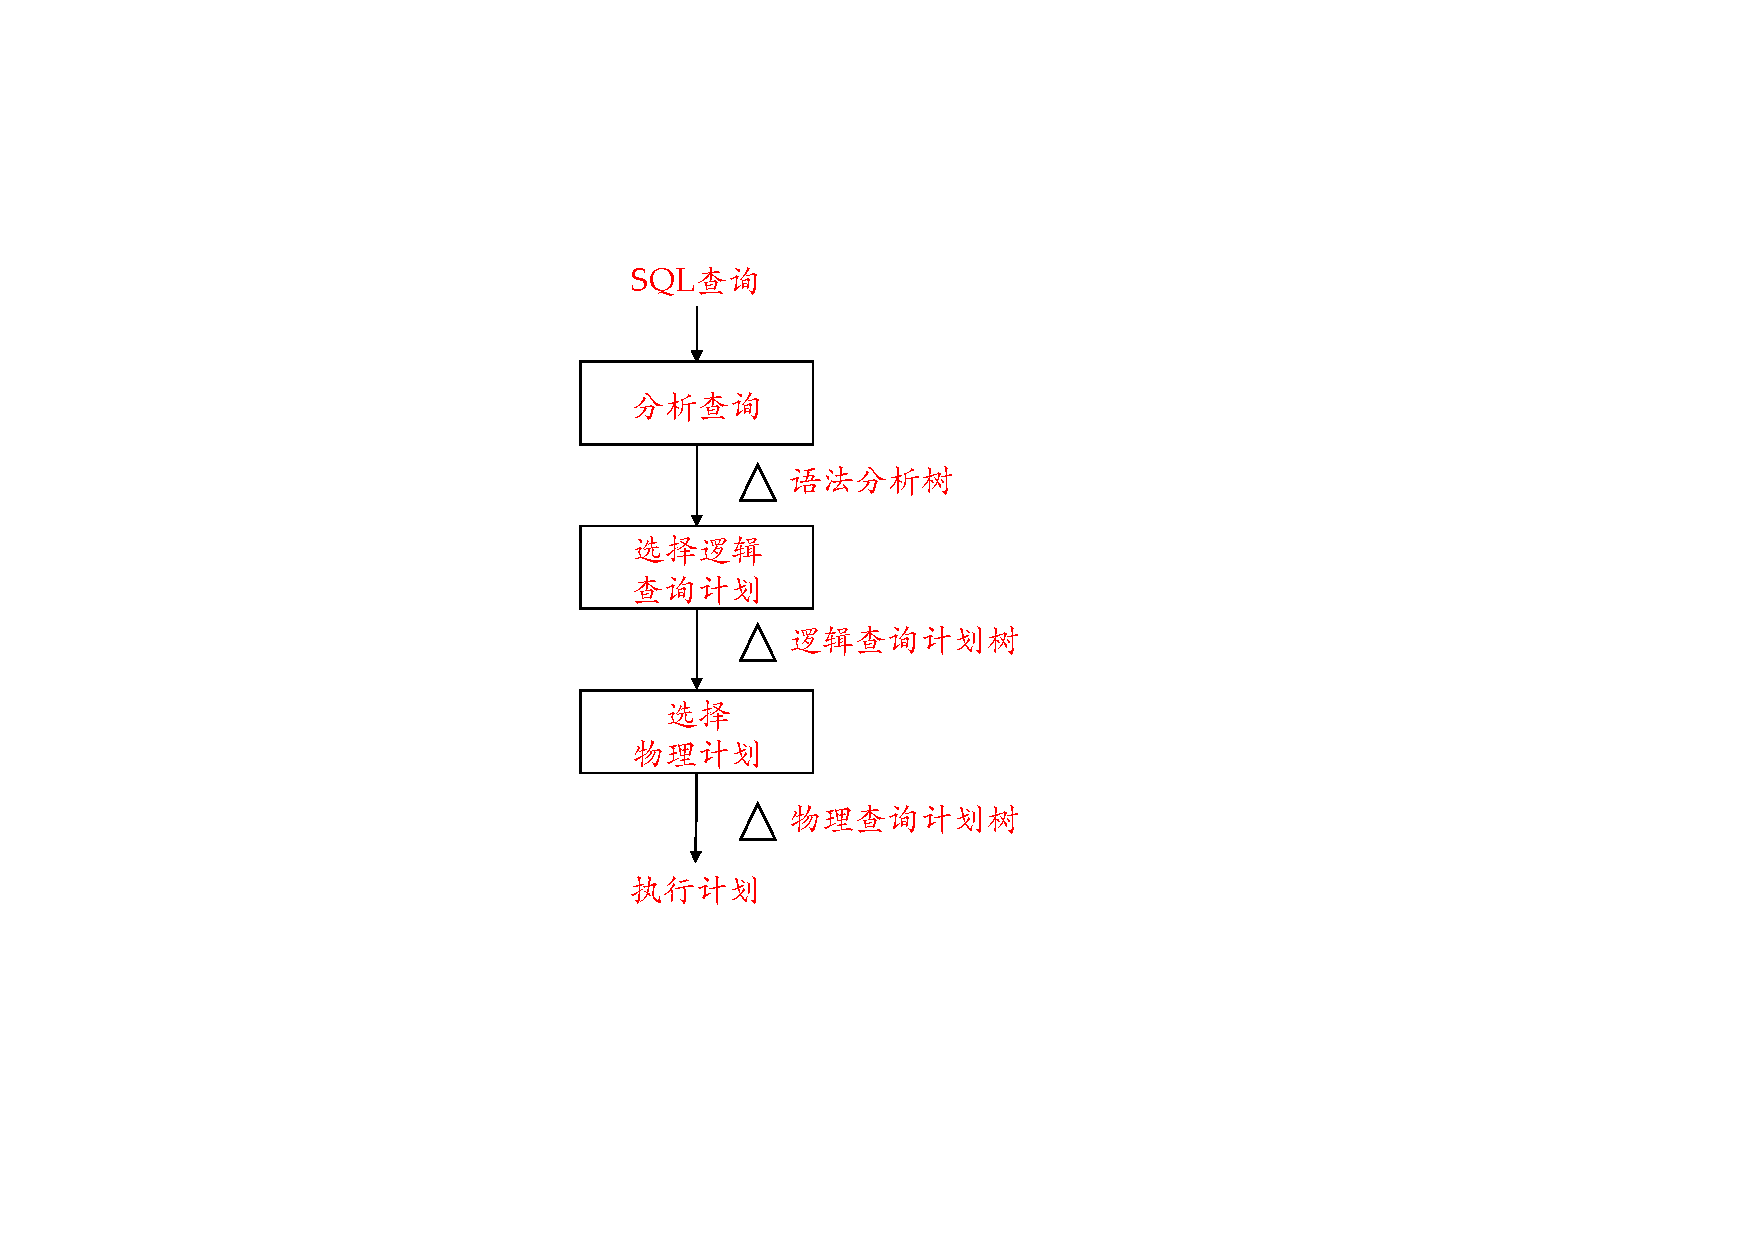
\includegraphics[width=.8\textwidth]{figure/chaxun.pdf}
    \caption{查询处理步骤}
\end{figure}

\subsection{查询优化}

\begin{definition}[查询优化]
    查询优化: 对一个给定的查询, 从多种可能执行方式中选择出最有效率的作为查询执行计划.
\end{definition}

高效的执行计划有两方面的衡量标准:
\begin{itemize}
    \item 使中间结果最小化
    \item 采用尽可能好的操作算法
\end{itemize}

\begin{definition}[基于代价的方法(cost-based)]
    基于代价的方法(cost-based): 
    \begin{itemize}
        \item 生成所有可能的侯选计划, 通过统计信息和存取路径确定每一计划中各个操作的代价和综合代价, 最后选择代价最小的一个;
        \item 优化代价较大.
    \end{itemize}
\end{definition}

\begin{definition}[启发式方法(rule-based)]
    启发式方法(rule-based):
    \begin{itemize}
        \item 主要是代数优化, 依据关系代数的等价变换做一些逻辑变换;
        \item 假定因素太多, 优化的代价虽小, 但优化的准确程度较差.
    \end{itemize}
\end{definition}

两种方法结合起来使用: 利用启发式方法尽量减少侯选计划, 利用基于代价的方法准确地确定执行计划.

\textbf{关系代数表达式的优化}:

利用关系代数表达式的等价规则: 各种结合律、分配律、交换律
\textcolor{red}{
    \begin{itemize}
    \item 将选择运算尽可能移向叶节点;
    \item 将选择运算尽可能移向叶节点;
    \item 合并可能的投影操作.
\end{itemize}
}

\textbf{查询代价}:
\begin{itemize}
    \item 查询处理对各种资源的使用情况
    \begin{itemize}
        \item 磁盘存取(简化为磁盘块传送数)
        \item CPU时间
        \item 通信开销
    \end{itemize}
    \item 一个重要的影响因素: 主存中缓冲区的大小M
    \begin{itemize}
        \item 最好的情形, 所有的数据可以读入到缓冲区中
        \item 最坏的情形, 缓冲区只能容纳数目不多的数据块
    \end{itemize}
\end{itemize}

\subsection{代价估算}

\begin{table}[H]
\centering
\begin{tabular}{|p{5cm}|p{10cm}|}
\hline
\textbf{访问方法} & \textbf{估计代价(逻辑读的数量)} \\ \hline
表扫描 & 表所占用的全部数据页的数量 \\ \hline
聚簇索引 & 索引的高度 + 要扫描的页的数量(要扫描的页的数量 = 满足条件的行的数量/每个数据页所包含的行的数量) \\ \hline
堆上的非聚簇索引 & 索引的高度 + 叶结点所指的页面数 + 满足条件的行的数量(可能所有的行均不在同一页中,所以要得到一行就必须要一次逻辑读).由于相同的数据页经常要读取多次(从缓冲区中读取),所以这样逻辑读的数量将比表的页面数要多 \\ \hline
聚簇索引上的非聚簇索引 & 索引的高度 + 叶结点所指的页面数 + (满足条件的行的数量×搜索一个聚簇索引码的代价) \\ \hline
非聚簇覆盖索引 & 索引的高度 + 索引的叶结点所占用的索引页(满足条件的行数/每个叶页面包含的行数) \\ \hline
\end{tabular}
\caption{不同访问方法的估计代价}
\label{tab:access_methods_cost_simple}
\end{table}

\subsection{统计信息}

关系 $R$ 的统计信息:
\begin{itemize}
    \item $T(R)$: $R$中的元组数
    \item $S(R)$: $R$中每个元组的字节数
    \item $B(R)$: $R$中所有元组所占据的块数
    \item $V(R, A)$: $R$的属性$A$上的唯一值的个数
    \item $f(R)$: 每个块上的$R$中元组的最大数目
\end{itemize}

索引 $I$ 的统计信息:
\begin{itemize}
    \item $HT(i)$: 索引的层数
    \item $LB(i)$: 索引叶结点的块数
\end{itemize}

数据库系统通常会维护一些系统表或数据字典, 用来存储与数据库对象(如表、索引等)相关的统计信息, 这就是\textcolor{red}{Statistics字典表}, 使用 \verb|ANALYZE TABLE| 命令触发.

\begin{lstlisting}[language=SQL, caption={基于规则的优化示例}]
create table test (col1 unique, col2)
select col1, sum(col2)
group by col1
\end{lstlisting}

上面的代码中, 由于col1是unique的, 所以系统并不执行分组操作.

\section{执行计划}

\subsection{数据查找}

\textbf{堆上的表}:

\begin{figure}[H]
    \centering
    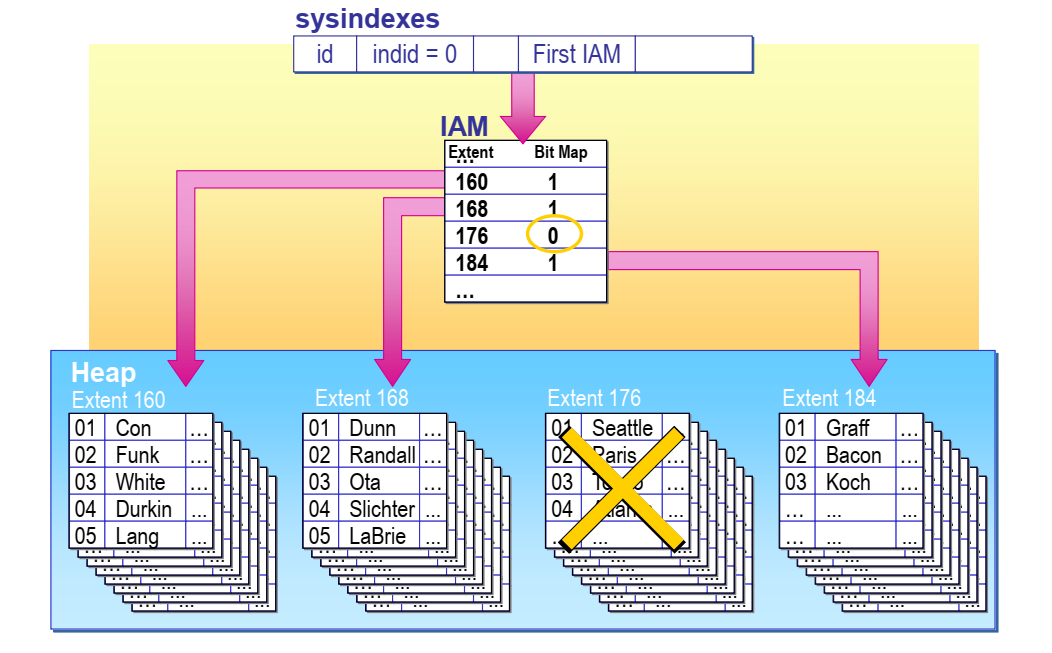
\includegraphics[width=.7\textwidth]{figure/堆上的表.png}
    \caption{堆上的表}
\end{figure}

聚簇索引(Clustered Index)是指数据库表中数据行的物理存储顺序与某一索引的键值顺序一致, 也就是说, 聚簇索引决定了表中数据的物理排列方式. 因为数据在磁盘上的存储顺序是按照聚簇索引的键值排序的, 所以一个表只能有一个聚簇索引.

\begin{figure}[H]
    \centering
    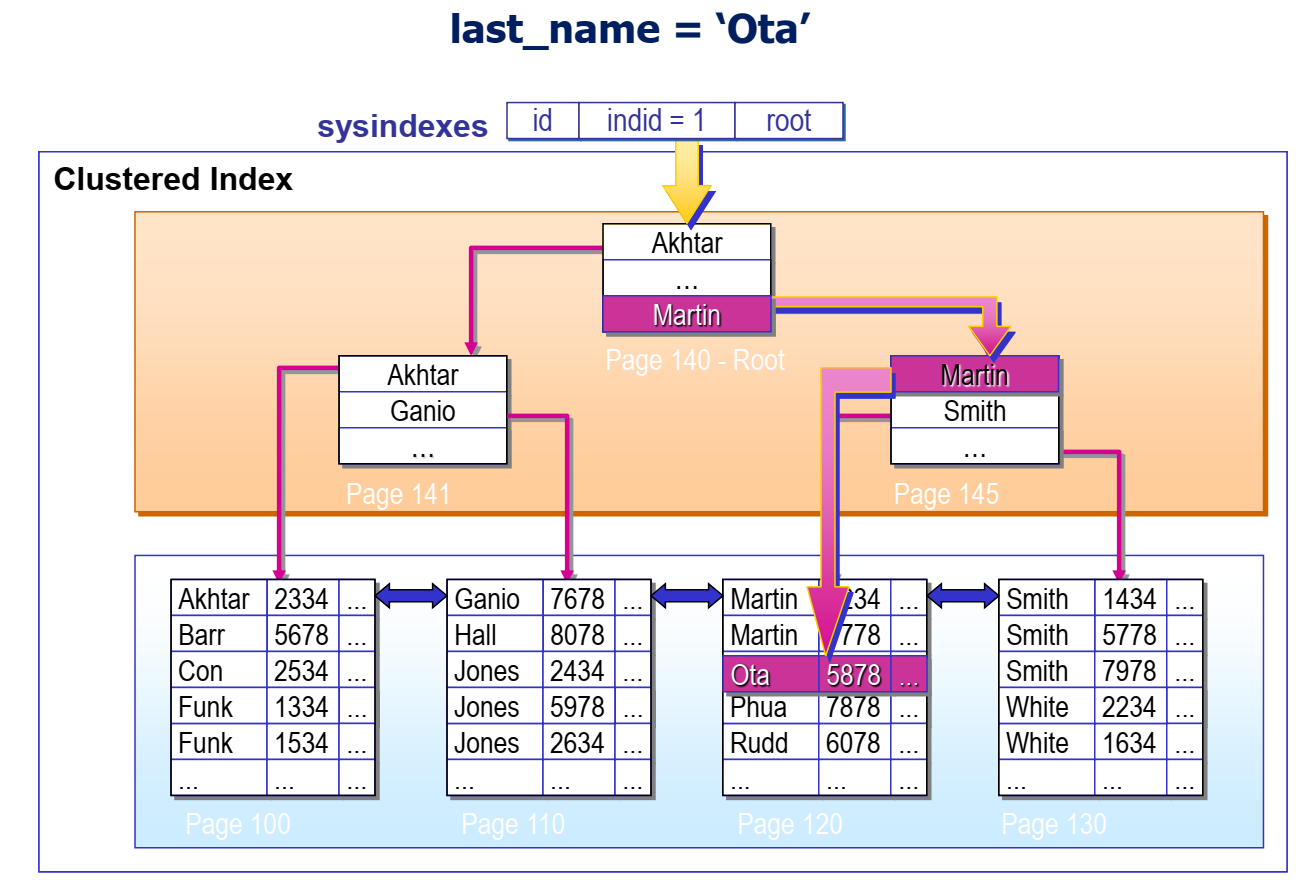
\includegraphics[width=.7\textwidth]{figure/聚簇索引.png}
\end{figure}

\textbf{堆上的非聚簇索引表结构}

\textbf{聚簇索引表上的非聚簇索引}

"Unimportant. There's a million things that I haven't done."

\subsection{各种访问方法}

对于关系$R(A, B, C, P)$:
\begin{itemize}
    \item 表扫描: \verb|select * from R|. 整张表的扫描, 开销是100\%.
    \item 无序聚簇索引扫描: \verb|select * from R|. \verb|create clustered index cidx1 on R(P)|. 虽然按照一定顺序扫描, 但是依然是整张表的扫描, 开销是100\%.
    \item 有序聚簇索引扫描
    \item 无序覆盖非聚簇索引扫描
    \item 有序覆盖非聚簇索引扫描
    \item 非聚簇索引查找 + 有序局部扫描 + Lookups
    \item 索引交集
\end{itemize}

"Unimportant. There's a million things that I haven't done."


\section{算子实现}

每一个基本的代数运算都有多种不同的实现算法, 适用于不同的情况
\begin{itemize}
    \item 等值条件, 范围条件
    \item 数据是聚集的, 数据是非聚集的
    \item 相关属性上有索引, 相关属性上没有索引
    \item 执行代价不同
\end{itemize}

\begin{figure}[H]
    \centering
    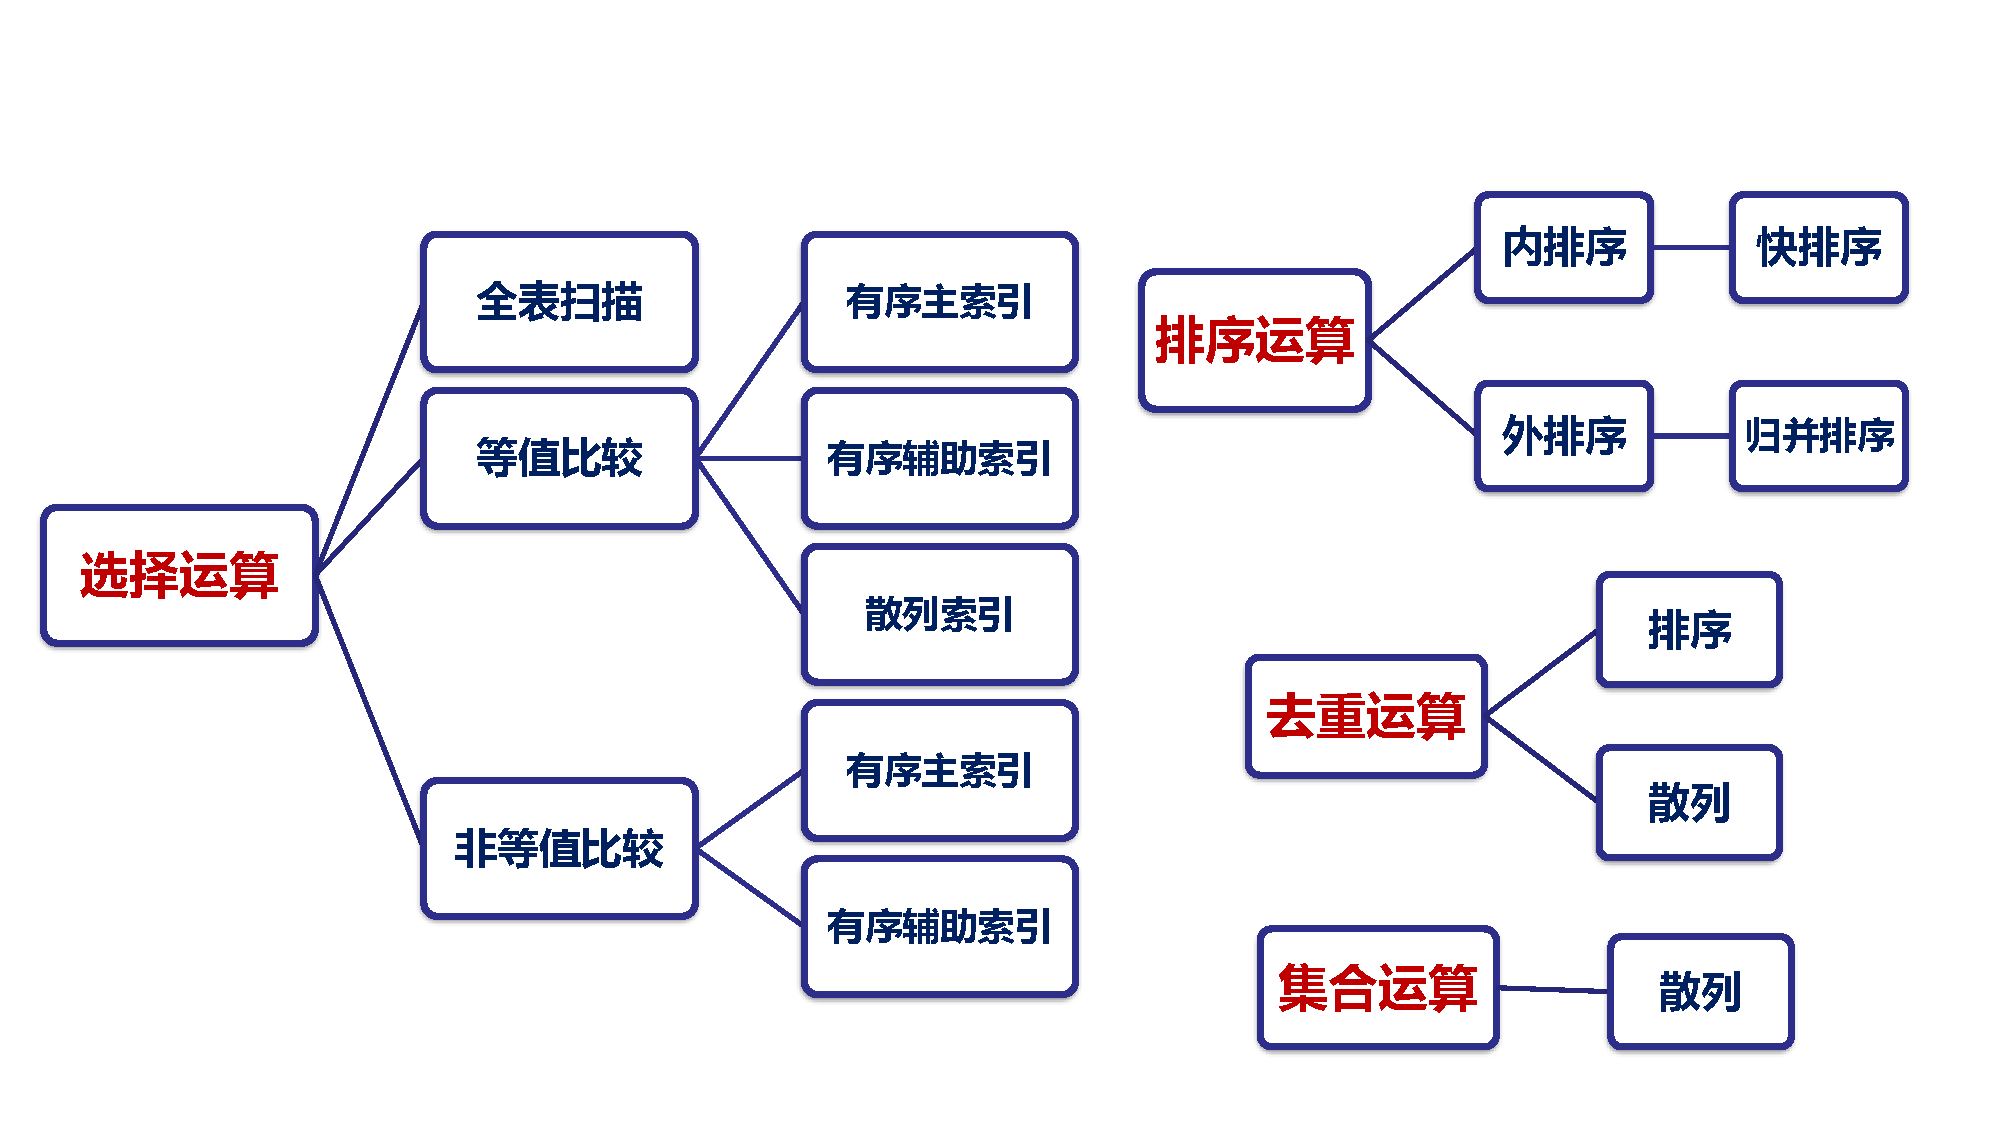
\includegraphics[width=.8\textwidth]{figure/物理算子-1.pdf}
    \caption{实现各种逻辑运算的物理算子概览}
\end{figure}

\begin{figure}[H]
    \centering
    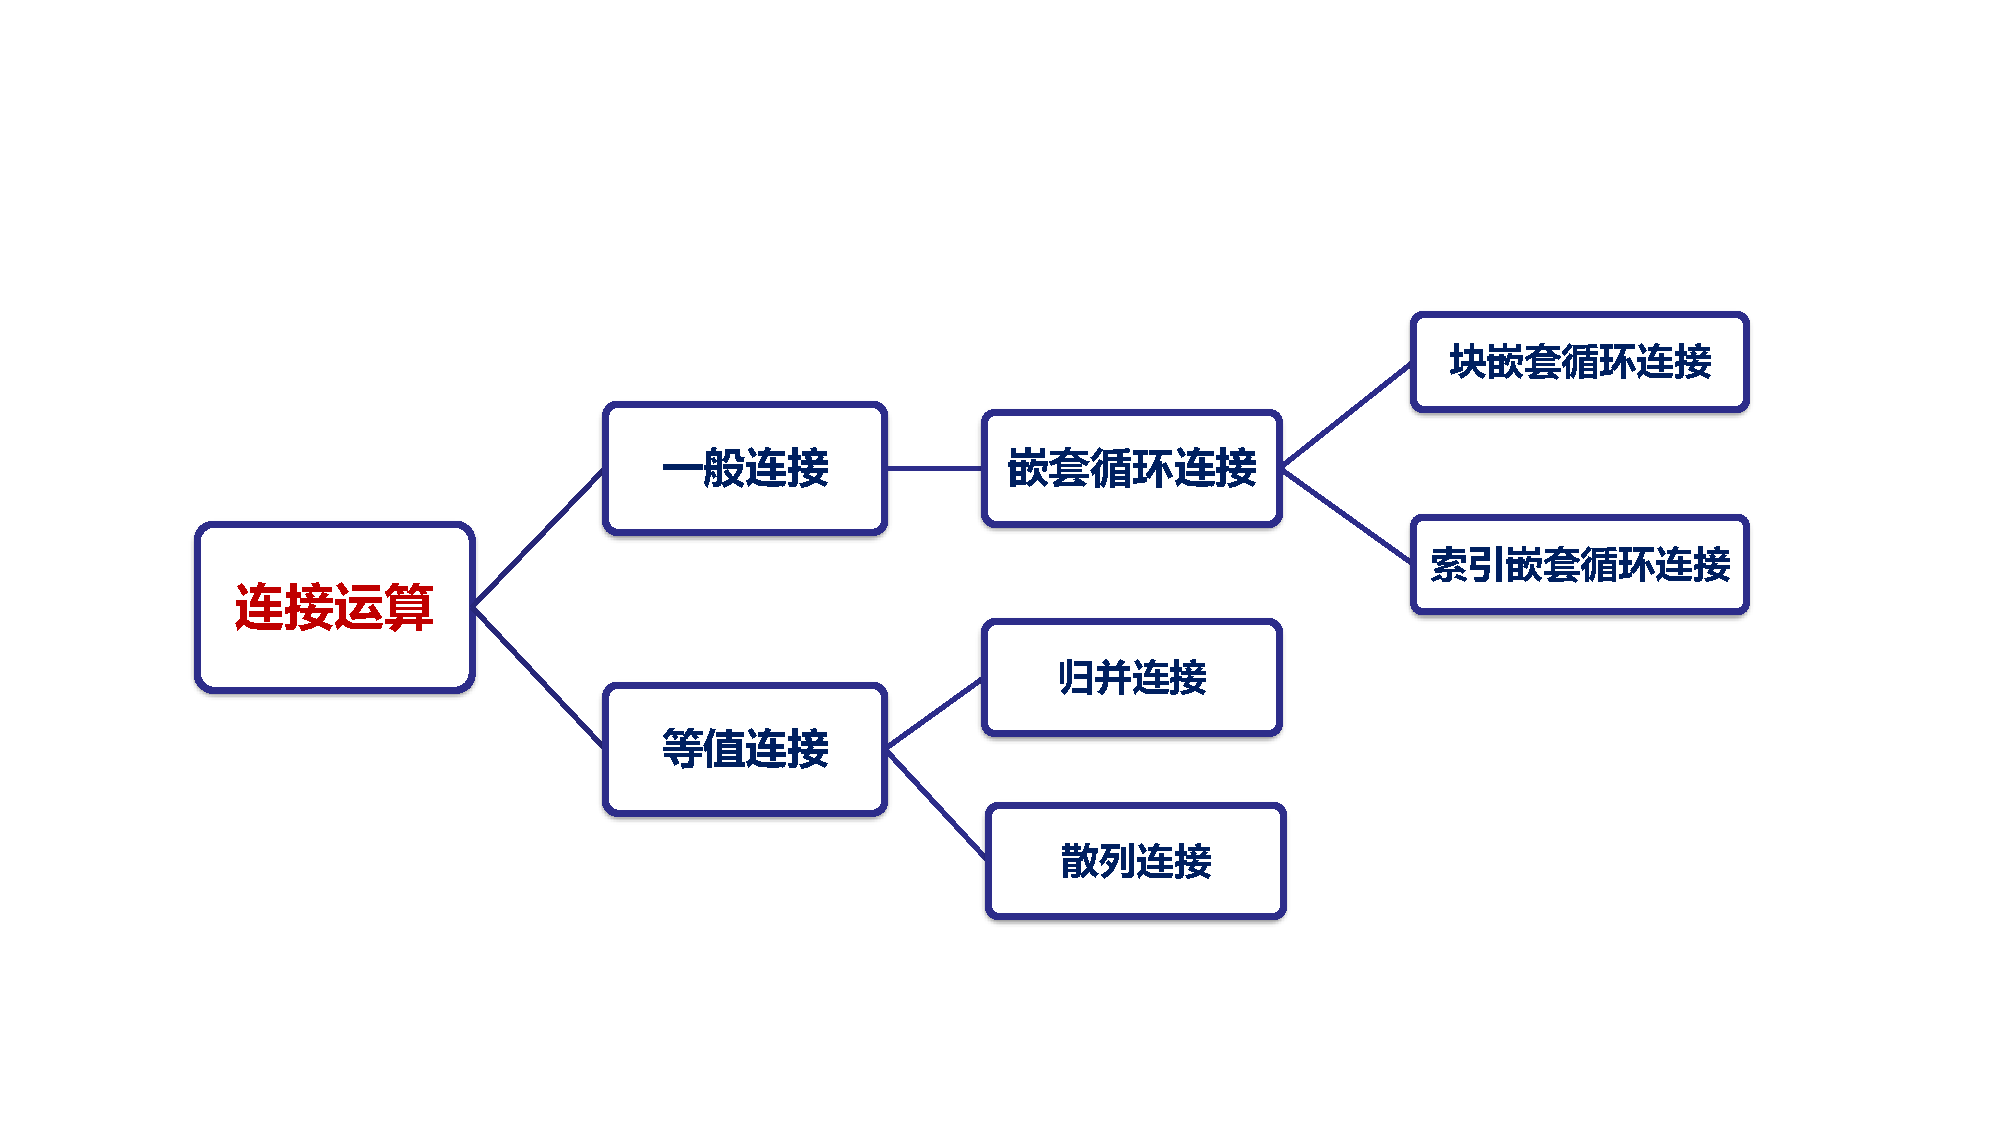
\includegraphics[width=.7\textwidth]{figure/物理算子-2.pdf}
    \caption{实现各种逻辑运算的物理算子概览}
\end{figure}

\subsection{选择运算}

\textbf{全表扫描}:
\begin{itemize}
    \item 方法: 依次访问表的每一个块, 对于每一个元组, 测试它是否满足选择条件
    \item 代价: $B(R)$, 如果是码查找, 平均代价为$B(R)/2$, 因为主码只有一个, 平均下来只要查找一半的长度
    \item 缺点: 效率低
    \item 优点: 对关系的存储方式没有要求, 无需索引
    \item 适用于任何选择条件
\end{itemize}

\textbf{等值比较选择$\sigma_{A=v}(r)$:}
\begin{itemize}
    \item 利用有序主索引.
    \begin{itemize}
        \item 在B+树索引中找到相应的叶结点, 其中包含指向满足该等值条件的记录的一个或多个指针. (满足条件的记录在一个块或相邻的多个块中)
        \item 代价: I/O操作次数等于B+树的高度, 加上包含具有搜索码值的记录的磁盘块数
    \end{itemize}
    \item 利用有序辅助索引.
    \begin{itemize}
        \item 在B+树索引中找到相应的叶结点, 其中包含指向满足该等值条件的记录的一个或多个指针. (满足条件的记录在不相邻的多个块中)
        \item 代价: I/O操作次数等于B+树的高度, 加上检索到的记录数目
    \end{itemize}
    \item 散列索引.
    \begin{itemize}
        \item 通过计算散列函数找到相应的桶, 在桶中检索到满足该等值条件的一条或多条记录
        \item 代价: I/O操作次数等于到桶的定位, 加上存储桶所包含的块数
    \end{itemize}
\end{itemize}

\textbf{非等值比较选择$\sigma_{A>v}(r)$:}
\begin{itemize}
    \item 利用有序主索引.
    \begin{itemize}
        \item 在索引中查找$v$值以检索出满足条件$A=v$的首条记录. 从该元组开始到文件尾进行文件扫描返回所有满足$A>v$条件的元组.
        \item 代价: I/O操作次数等于B+树的高度, 加上包含满足搜索条件的记录的磁盘块数
    \end{itemize}
    \item 利用有序辅助索引.
    \begin{itemize}
        \item 在索引中查找$v$值以检索出满足条件$A=v$的首条记录. 从该索引条目直至最大值索引条目提供了指向满足条件的记录的指针, 根据指针逐个取实际记录
        \item 代价: I/O操作次数等于B+树的高度, 加上包含满足搜索条件的记录的磁盘块数
    \end{itemize}
\end{itemize}

\subsection{排序}

排序场合:
\begin{itemize}
    \item SQL查询可以指定对输出进行排序
    \item 关系运算的某些操作, 如连接运算, 排序后实现高效
\end{itemize}

对于可放进内存的关系, 使用如快排序之类的技术.

对不能放进内存的关系, \textcolor{red}{使用外排序.}
\begin{itemize}
    \item 外排序: 创建有序段 + $N$路归并
    \item 所有的输入数据最初分成许多有序的归并段文件, 然后不断归并成许多更大的归并段文件, 直到剩下一个文件为止
\end{itemize}

\subsection{集合运算}

相同的散列函数对两个关系进行划分, 由此得到各个划分, 对关系$r$的一
个划分建立内存中的hash索引, 然后针对每一个划分进行以下的步骤:
\begin{enumerate}
    \item 并: 把$s$中相应划分中的元组加入以上的hash索引中, 条件是元组不在hash索引中, 把hash索引中的元组加入到结果中
    \item 交: 对$s$中相应划分中的每一个元组, 检索hash索引, 若它出现在其中, 就将该元组写入结果
    \item 差: 对关系$s$相应划分中的每一个元组, 检索hash索引, 若它出现在其中, 就将它从hash索引中删除. 将hash索引中剩余的元组加入结果中
\end{enumerate}

\subsection{去重}

\begin{enumerate}
    \item 用排序的方法.
    \begin{itemize}
        \item 创建归并段文件时可以发现重复元组, 并在将归并段文件写回磁盘之前去除重复元组, 从而减少块传输次数
        \item 归并时再去除剩余的重复元组
    \end{itemize}
    \item 用散列的方法
    \begin{itemize}
        \item 基于整个元组上的一个散列函数对关系进行划分
        \item 每个分划被读入内存, 建立内存中的散列索引
        \item 建立散列索引时, 只有不在索引中的元组才被插入. 否则, 元组就被抛弃. 分划中的所有元组处理完后, 散列索引中的元组被写到结果中
    \end{itemize}
\end{enumerate}

\subsection{连接运算}

\begin{itemize}
    \item 嵌套循环连接
    \item 块嵌套循环连接
    \item 索引嵌套循环连接
    \item 归并连接
    \item 散列连接
\end{itemize}


$r$ 称为连接的外关系,$s$ 称为内关系

\textbf{嵌套循环连接}: \textcolor{red}{不需要索引, 可用于任何连接条件.}

\begin{algorithm}[H]
    \KwIn{关系 $r$ 和 $s$, 连接条件 $\theta$}
    \KwOut{连接结果 $r \bowtie_{\theta} s$}
    
    \For{每个元组 $t_r$ 属于 $r$}{
        \For{每个元组 $t_s$ 属于 $s$}{
            测试元组对 $(t_r, t_s)$ 是否满足连接条件 $\theta$\;
            \If{$(t_r, t_s)$ 满足连接条件 $\theta$}{
                将 $t_r \cdot t_s$ 加入到结果中\;
            }
        }
    }
    \caption{嵌套循环连接}
\end{algorithm}

\textbf{块嵌套循环连接}: \textcolor{red}{在外层循环中使用较小的关系代价略小.}
\begin{itemize}
    \item 当较小的关系放在外层循环时, 每次外层循环迭代时, 只需要加载较少的数据到内存中进行处理. 这减少了磁盘 I/O 操作的次数, 从而提高了整体性能.
    \item 相反, 如果较大的关系放在外层循环中, 每次外层循环迭代时都需要加载大量的数据到内存中, 增加了 I/O 开销.
\end{itemize}

\begin{algorithm}[H]
    \KwIn{关系 $r$ 和 $s$, 连接条件 $\theta$}
    \KwOut{连接结果 $r \bowtie_{\theta} s$}
    \For{每个块 $B_r$ 属于 $r$}{
        \For{每个块 $B_s$ 属于 $s$}{
            \For{每个元组 $t_r$ 在 $B_r$}{
                \For{每个元组 $t_s$ 在 $B_s$}{
                    检查 $(t_r, t_s)$ 是否满足连接条件\;
                    \If{$(t_r, t_s)$ 满足连接条件}{
                        将 $t_r \cdot t_s$ 加入结果\;
                    }
                }
            }
        }
    }
    \caption{块嵌套循环连接}
\end{algorithm}


\textbf{索引嵌套循环连接}:
\begin{itemize}
    \item 如果满足下列条件, 索引查找可以代替文件扫描
    \begin{itemize}
        \item 是等值连接或自然连接
        \item 在内关系的连接属性上存在索引
    \end{itemize}
    \item 对外关系$ r $的每个元组 $t_r$, 利用索引查找内关系 $s$ 的与 $t_r$ 满足连接条件的元组
\end{itemize}

\textbf{归并连接}: 用于执行两个关系之间等值连接操作的高效算法, 尤其适用于已经排序的数据. 其基本思想是将两个输入关系按照连接属性进行排序, 然后通过同步扫描这两个关系来找到满足连接条件的元组对.

\begin{algorithm}[H]
    \KwIn{关系 $r$ 和 $s$}
    \KwOut{连接结果 $r \bowtie_{r.A = s.A} s$}
    
    初始化指针 $i = 1$, $j = 1$\;
    
    \While{仍有未处理的块或元组}{
        在 $r$ 和 $s$ 的当前块中查找连接属性的最小值 $v$\;
        
        \If{$v$ 在另一关系的当前块中不存在}{
            删除具有该值的所有本地元组\;
            移动指针以跳过这些元组\;
        }
        \Else{
            收集 $r$ 和 $s$ 中所有连接属性等于 $v$ 的元组\;
            \If{某关系当前块不够, 需更多元组}{
                从磁盘加载下一个包含该值的块\;
            }
            
            执行局部笛卡尔积, 生成连接结果\;
            输出所有符合条件的结果元组\;
            
            \If{某关系当前缓冲区无可用元组}{
                重新加载该关系的缓冲区\;
            }
        }
    }

    \caption{归并连接算法}
\end{algorithm}

\textbf{散列连接}:
\begin{itemize}
    \item 适用于自然连接和等值连接
    \item 基本思想
    \begin{itemize}
        \item 将两个关系按连接属性值划分成有相同散列函数值的元组集合
        \item 关系$r$在一个散列划分中的元组只需要与关系$s$在对应的划分中的元组相比较
        \item 在$r$和$s$的每一对划分中进行索引嵌套循环连接(或者散列连接)
    \end{itemize}
\end{itemize}

\begin{figure}[H]
    \centering
    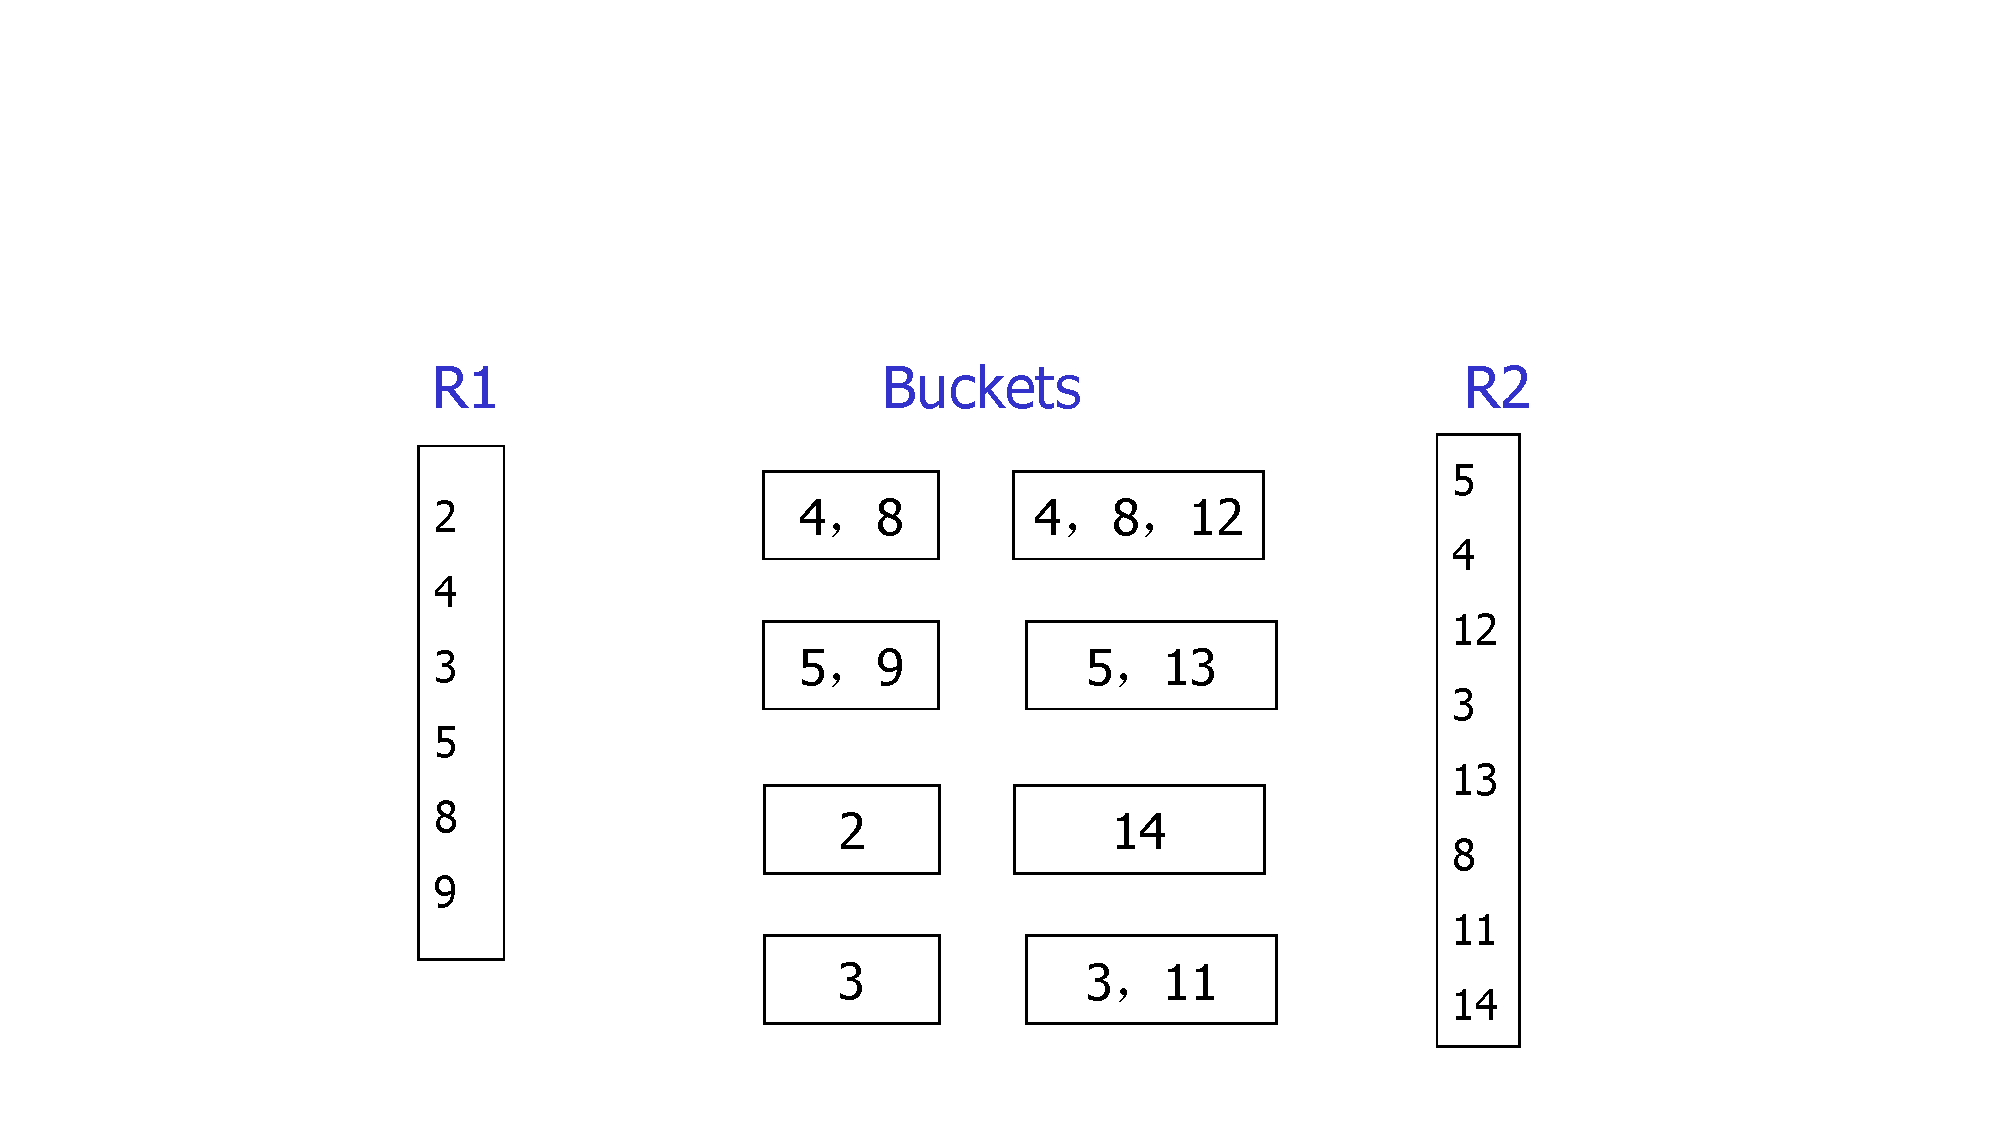
\includegraphics[width=.5\textwidth]{figure/散列连接.pdf}
    \caption{散列连接示例}
\end{figure}

\textbf{总结比较}
\begin{itemize}
    \item 如果一个连接输入很小(比如不到 10 行), 而另一个连接输入很大而且已在其连接列上创建索引, 则索引嵌套循环是最快的连接操作
    \item 如果两个连接输入很大, 并已在二者连接列上排序(连接列上有索引), 则合并连接是最快的连接操作
    \item 哈希连接可以处理很大的、未排序的非索引输入
    \item 如果两个连接输入都很大, 而且这两个输入的大小差不多, 则预先排序的合并连接提供的性能与哈希连接相似. 然而, 如果两个输入的大小相差很大, 则哈希连接操作通常快得多
    \item 合并连接和哈希连接只能用于等值连接, 对于非等值连接, 只能用嵌套循环连接
\end{itemize}

\subsection{多表连接}

$N$个表可能的连接种类有$N!$个

\begin{itemize}
    \item 对少于或等于4个的表连接采用验证全部组合的方法, 对于超过4个的表连接, 以4个表为一组进行验证.
    \item ABCDEF6个表, 先求出其任意4个表组合中代价最小的, 不妨设为BCDF, 则表B作为最外层表, 剩余5个表ACDEF, 再求出其任意4个表组合中代价最小的, 不妨设为CDEF, 则表C作为次外层表, 最后按通常方法确定剩余表的最佳连接顺序, 假设为DEFA, 则最后表连接顺序为BCDEFA
\end{itemize}

\subsection{算子执行方式}

\begin{definition}[物化执行(Materialization)]
    物化执行(Materialization):
    \begin{itemize}
        \item 生成输入为关系或已计算结果的表达式的结果, 在磁盘上物化(存储)
        \item 从最底层开始每次计算一个运算, 将中间结果物化成临时关系, 再进行下一层运算
        \item 物化执行总是可用的
        \item 将结果写到磁盘并读回来可能代价很高
    \end{itemize}
\end{definition}

\begin{definition}[流水线化(Pipelining)]
    流水线化(Pipelining):
    \begin{itemize}
        \item 当一个操作正在执行中, 就将部分输出元组送到父运算
        \item 流水线执行: 同时计算多个运算, 将一个运算的结果传到下一个运算
        \item 比物化执行代价要低, 不需要将临时关系存储到磁盘
        \item 有时流水线不可用 - 如排序和散列连接
        \item 为了使流水线有效, 使用能在接受输入元组的同时生成输出元组的执行算法(无阻塞算子)
    \end{itemize}
\end{definition}

\subsection{算子封装形式: 迭代器}

\begin{itemize}
    \item open(): 打开一个输入
    \item getnext(): 一次一个项的读取每一个项, 如果遇上一个项符合条件的话, 就将这个项传递给下一个处理迭代器
    \item close(): 关闭输入
\end{itemize}